\subsection{Code example}

In this section, we introduce the reader to a simple example program of Jolie. The program emphasizes the capability of the module system by interchanging a service through common interface operation.  

The following code snippet is a hello-world example of the Jolie module system.

\begin{listing}[H]
    \lstset{language=Jolie,
        style=codeStyle,
        numbers=left,
        firstnumber=1
    }
    \begin{lstlisting}[frame=tlrb]{service-hello.ol}
from console import ConsoleService, ConsoleInterface

service main(){

    outputPort Console {
        interfaces: ConsoleInterface
    }

    embed ConsoleService() in Console

    main{
        print@Console("Hello")()
    }
}
\end{lstlisting}

\end{listing}

At line 1, we have an import statement to import the ConsoleService along with the interface exposed by its service. The ConsoleService is a build-in service that allows a Jolie program to communicate to the execution process system console. Afterwards, we declare a service node called main, with an outgoing communication Console that uses an operation in ConsoleInterface. At line 9, The communication port Console is later bound with the service ConsoleService through the embed statement. It resulted in an usable Console port which communicates internally with ConsoleService, without specification on the location or protocol parameter in its declaration.
In the main procedure, we invoke the operation \textit{print} through the output port Console. Executing this program results in \say{Hello} being printed at the process console.

\subsubsection{Service Injection Pattern}

Our last example describes a way to compose a simple service in the Jolie module system. Here, we can extend the previous example to an advanced scenario. Given a situation where we want to have our own workflow on the operation \textit{print}. We create a new service, \textit{PrinterService}, which exposes the operation \textit{print}, with a simple workflow of prefixing an incoming message before forwarding it to the system console.

\begin{listing}[H]
    \lstset{language=Jolie,
        style=codeStyle,
        numbers=left,
        firstnumber=1
    }
    \begin{lstlisting}[frame=tlrb]{printer.ol}
from console import ConsoleService, ConsoleInterface

interface PrinterInterface {
RequestResponse:
    print( undefined )( void )
}

service PrinterService() {

    execution { concurrent }
    
    inputPort IP {
        location: "local"
        interfaces: PrinterInterface
    }

    embed ConsoleService in new _Console

    main{
        [print(req)(res){
            res = "Printer receive: " + req
            print@_Console(res)()
        }]
	// omitted code
    }
}
\end{lstlisting}
\end{listing}

\begin{listing}[H]
    \lstset{language=Jolie,
        style=codeStyle,
        numbers=left,
        firstnumber=1
    }
    \begin{lstlisting}[frame=tlrb]{service-injection-hello.ol}
from console import ConsoleInterface
from .printer import PrinterService

service main(){

    outputPort Console {
        interfaces: ConsoleInterface
    }

    embed PrinterService() in Console

    main{
        print@Console("Hello")()
    }
}
\end{lstlisting}
\end{listing}

After the service has been defined, we only have to import and embed the \textit{PrinterService} instead of \textit{ConsoleService} of our last example. The client of this service will now use the operation \textit{print} of the \textit{PrinterService} and program results in \say{Printer receive: Hello} being printed.

Since the operation \textit{print} is commonly exposed by both services, thus, these two services are interchangeable for the operation \textit{print}. 

The module system extends the flexibility of Jolie services and allows the service developer to create a new system in a modular approach. In the next section, we will look at the practical Jolie module system implementation of the Circuit Breaker, which is one of the prominent microservices patterns \cite{nygard2007release}.

\FloatBarrier

\subsubsection{Microservice Pattern: Circuit Breaker}

In this section, we discuss an implementation of the circuit breaker pattern in Jolie and emphasize Jolie’s capability as a language for microservices. After the discussion on implementation source code, we also explore the integration of this application with the container technology, particularly Docker container.

The circuit breaker is a well-known pattern in the microservice architecture \cite{martin-2015-circuit, microservices.io-circuit}. It enables an application to proceed on a request properly on the situation of an arbitrary dependent service that has failed to progress. A possible application scenario of circuit breaker is where a network of services communicate with each other to build up a client’s response, and one of the services is taking a longer-than-usual processing time. This processing time can be a result of network latency. Otherwise, there might be a failure during the processing of a task, which cannot be foreseen by other services. The pattern increases the fault-tolerant of the whole system by monitoring the service behavior and prevents an unexpected failure from cascading to other services by performing a cutout action, just like the circuit breaker in the physical world.

A circuit breaker implementation in the microservices ecosystem is a proxy service between clients to a service. The circuit breaker monitors the request and counts the number of failures that happens through calls made to the destination service. If the number of failures reaches the threshold, it discards and returns a meaningful response for the client without attempting to make a call to the destination service. Later after a certain amount of time, on the invocation to the service, the circuit breaker slowly forwards the request again.

There are three states in circuit breaker which determine the state of calls made to the destination service. Firstly, the \textit{Closed} is a healthy state of the circuit breaker. At this state, every request for an operation will be passed to the service. Each failure occurred from the call, either internally from the service or the request timeout, the circuit breaker increases the counter.When the number of failures reaches the threshold number, the circuit breaker trips by changing its state to \textit{Open} and start a reset timeout. At this state, any request made to the destination operation is skipped by the circuit breaker as it is presumed that the destination service is down. The developer of the circuit breaker can design the fallback procedure, for example, return a cached response to the client or straightforwardly return an error response. After the reset timeout ticks, the circuit breaker changes its state to \textit{Half-Open}, where any call will be passed to the destination service. If the service responds without any error, the circuit breaker sets its state to \textit{Closed} or in a healthy state. Otherwise, the circuit breaker falls back to status \textit{Open} again. The states for a circuit status illustrate in the figure\ref{figure:circuit-breaker-state-diagram}. 

\begin{figure}
    \centering
    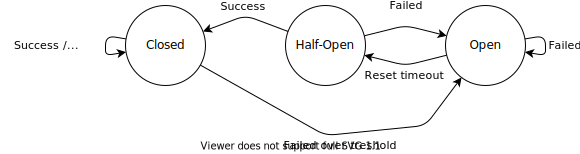
\includegraphics[width=\textwidth]{Doc-images-circuit-breaker.pdf}
    \caption{State diagram for circuit breaker service}
    \label{figure:circuit-breaker-state-diagram}
\end{figure}

Montesi and Weber have studied the implementation of circuit breaker pattern for Jolie application\cite{10.1145/3167132.3167427}, which extends a decorator pattern and sketches an implementation of circuit breaker pattern in Jolie. In our version, we exploit the capability of importing service to extend a single service with a circuit breaker extension service. We begin with a circuit breaker service, which is implemented as an extension service to be imported and embedded by others. We firstly define types and interfaces definitions for the circuit breaker, which is shown in figure.

Start with a circuit breaker service, which is implemented as an extension service to be imported and embedded by others. We firstly define types and interfaces definitions for the circuit breaker, as shown in figure ~\ref{list:circuit-breaker-def}. We required three interfaces for handling the operation as followed:
\begin{itemize}
    \item the \texttt{HTTPInterface} defines an operation for handling an communication between the circuit breaker to the client.
    \item The \texttt{CircuitBreakerServiceCallbackInterface}, defines an operation for handling an communication between the circuit breaker to the destination service.
    \item Lastly, \texttt{CircuitBreakerInternalInterface} defines the internal operation such as timeout for resetting the Opened state and request timeout handler. 
\end{itemize}

The client requests are handled through an HTTP protocol with a special configuration \textit{default}, which will be invoked as a default operation when the undefined operation is passed to the service.  field by assigning the service parameter. Figure ~\ref{list:circuit-breaker-component-diagram} demonstrated the interfaces exposed by the circuit breaker service.

\begin{figure}
    \centering
    \includegraphics[width=\textwidth]{Doc-images-circuit-breaker-service.pdf}
    \caption{Component diagram for the circuit breaker service}
    \label{list:circuit-breaker-component-diagram}
\end{figure}

Furthermore, we also define a type for configuring the service. As a proxy service, we require additional input from the embedder service, the exposing input location, and the target location. 
It is worth mentioning that we give the responsibility to importer service to configure \textit{location} of the communication channel. The source code for what we have mentioned so far is shown at figure ~\ref{list:circuit-breaker-def}

\renewcommand{\topfraction}{.85}
\renewcommand{\bottomfraction}{.7}
\renewcommand{\textfraction}{.15}
\renewcommand{\floatpagefraction}{.66}
\renewcommand{\dbltopfraction}{.66}
\renewcommand{\dblfloatpagefraction}{.66}
\setcounter{topnumber}{9}
\setcounter{bottomnumber}{9}
\setcounter{totalnumber}{20}
\setcounter{dbltopnumber}{9}

\begin{listing}[]
    \lstset{language=Jolie,
        style=codeStyle,
        basicstyle=\ttfamily\footnotesize
    }
    \begin{lstlisting}[frame=tlrb]{circuitbreaker-definitions.ol}
interface HTTPInterface{
    requestResponse:
        default(undefined)(undefined)
}

interface CircuitBreakerServiceCallbackInterface{
    requestResponse: callback(undefined)(undefined) throws UnexpectedError(string)
}

private interface CircuitBreakerInternalInterface{
    oneWay: reset(undefined)
}

type CircuitBreakerServiceParam : void {
    inputLocation: string
    outputLocation: string
}

service CircuitBreakerService (p : CircuitBreakerServiceParam) { 
    inputPort HTTPInput {
        protocol: "http" {
            default = "default"
        }
        location: p.inputLocation
        interfaces: HTTPInterface
    }
    outputPort DestService {
        location: p.outputLocation
        protocol: "sodep"
        interfaces: CircuitBreakerServiceCallbackInterface
    }
    inputPort SelfInput{
        location: "local"
        interfaces: CircuitBreakerInternalInterface
    }
    ...
}
\end{lstlisting}
\caption{Definitions and communication ports for the circuit breaker service}
\label{list:circuit-breaker-def}
\end{listing}

Next as shown in figure ~\ref{list:circuit-breaker-workflow}, we define procedures and workflow for each operation exposed by the circuit breaker. The procedures included in this service encapsulate the actions made for state transformation. We use a global state, a shared state lived in every session initiated by the service, to store the counter of error number and the flag of the current status of the circuit breaker.

\begin{listing}[]
    \centering
    \lstset{language=Jolie,
        style=codeStyle,
        basicstyle=\ttfamily\footnotesize
    }
\begin{lstlisting}[frame=tlrb]{circuitbreaker-port.ol}
// constants declaration
service CircuitBreakerService (p : CircuitBreakerServiceParam) {
    ...
    define closeCircuit {
        global.errorCount = 0
        global.status = STATUS_CLOSED
    }
    define resetCircuit {
        global.status = STATUS_HALFOPEN
    }
    define trip {
        global.status = STATUS_OPEN
        scheduleTimeout@Time( TIMEOUT_REQUEST{.operation="reset"} )( )
    }
    define handleError {
        if (global.status == STATUS_HALFOPEN){
            trip
        } else if (global.errorCount > ERROR_THRESHOLD){
            trip
        }
    }
    init {
        closeCircuit
    }
    main {        
        [ reset() ]{
            resetCircuit
        }
        [ default( request )( response ) {
            if ( global.status == STATUS_OPEN ){
                response = "CircuitOpen"
            } else {
                install( UnexpectedError =>
                    global.errorCount++
                    handleError
                    response = "ServiceError"
                )
                callback@DestService(request)(serviceRes)

                if (global.status == STATUS_HALFOPEN){
                    closeCircuit
                }

                response << serviceRes
            }
        }]
    }
}
\end{lstlisting}
\caption{Workflow for circuit breaker service}
\label{list:circuit-breaker-workflow}
\end{listing}

The \textit{trip} procedure defines the instruction set to turn on the circuit, which is determined by procedure \textit{handleError}. After modifying the state, it proceeds with scheduling the timeout request for state recovery, defined in \textit{resetCircuit}, by invoking the operation from build-in service \textit{time}
\footnote{Time service specification \url{https://jolielang.gitbook.io/docs/language-tools-and-standard-library/standard-library-api/time}}.

The circuit breaker's initialization begins with a call to procedure \textit{closeCircuit}, which sets the state of the circuit to \textit{Closed} state. Later in the main execution, the service exposes and waits for two operations \textit{reset} and \textit{default}. The \textit{reset} operation is responsible for turn an Opened state of the circuit breaker to \textit{Half-Opened} by calling \textit{resetCircuit} procedure defined above. The operation for handling client requests, \textit{default}, as mention above, is invoked whenever the client is passing a message to the circuit breaker and forward the request to the destination service. The workflow of operation can be described as the following:
if the state of the circuit breaker, return a response without passing the request to destination service.
Otherwise, forward the request to destination service, if there is an error occurrence, call the error handling procedure and return a response to the client.

After we have defined the CircuitBreaker proxy service, which can be imported and embedded by any service, we look into an example service \textit{AddService}, which integrates the CircuitBreaker extension to handle the possible error that might occur internally.

\begin{listing}[]
    \lstset{language=Jolie,
        style=codeStyle,
        basicstyle=\ttfamily\footnotesize
        }
    \begin{lstlisting}[frame=tlrb]{circuitbreaker-client.ol}
from .circuitbreaker import CircuitBreakerService, CircuitBreakerServiceCallbackInterface

type input: void{
    x : int
    y : int
}

interface calculatorIface {
    requestResponse: 
        add(input)(int)
}

service main {
    
    // definition of self ports to redirect the request

    inputPort fromCircuitBreaker{
        location: "socket://localhost:3001"
        protocol: "http"
        interfaces: CircuitBreakerServiceCallbackInterface
    }

    embed CircuitBreakerService( { 
        inputLocation = "socket://localhost:3000"
        outputLocation = "socket://localhost:3001" 
    } )

    execution { concurrent }

    main{
        [add(req)(res){
		...
        }]
        [callback(req)(res){
            if (req.operation == "add"){
                add@SelfOp({x = int(req.data.x) y = int(req.data.y)})(response)               
            }       

		    if (error){
	    		throw ( UnexpectedError )
		    } else {
                res << response
         	}                  
        }]
    }
}
\end{lstlisting}
\caption{Jolie implementation of a service embedding the circuit breaker service}
\label{circuitbreaker-client.ol}
\end{listing}

Our implementation of the circuit breaker embedder, as shown in figure ~\ref{circuitbreaker-client.ol}, requires defining an operation \textit{callback}, which receives a message from the circuit breaker and redirect the request to proper operation. In this case, the workflow includes checking the request operation from \textit{operation} field then forward the message to an internal input port, defined using \textit{local} scheme for location. After the call is complete, return the corresponding result to the circuit breaker.

We had demonstrated an implementation of the microservice architecture, the circuit breaker, using the new feature of the module system. The Jolie module system enables Jolie developer to create and compose multiple sole responsibility services and create a more complex application using the import mechanism.